\documentclass[aps,prl,twocolumn, superscriptaddress,nobalancelastpage]{revtex4}
\usepackage{graphicx}
\usepackage{amssymb}
\usepackage{amsmath}
\usepackage{color}
\usepackage{academicons}
\usepackage{xcolor}



\begin{document}


\title{Subwavelength grating optical ring resonator devices for biosensing applications} 



\author{Daniel Hutama}
\author{Sam Lantela}
\author{Yeseul Lee}
\affiliation{Dept. of Electrical \& Computer Engineering, McGill University, Montr\'eal, Qu\'ebec, H3A 0E9, Canada}

\date{\today}
\begin{abstract}
\noindent \textbf{Abstract:}  One notable development in optical mircroring biosensors is the use of subwavelength grating (SWG) waveguides due to their increased sensitivity to index changes in the waveguide cladding material.  Ring devices based on SWG waveguides have substantial commercial potential due to their wide range of applications and compatibility with mainstream CMOS foundry processes.  Although such biosensors continue to see high levels of academic research activity, they have yet to make a large-scale breakthrough in commercialized frontline medical diagnostics equipment.  After presenting the operational principles of SWG ring biosensors and discussing the state-of-the-art in SWG ring-based biosensing, we present a comparison of various optical resonator designs. We conclude with a discussion of various design advantages, practical limitations, and challenges of silicon photonic biosensing devices.
\end{abstract}
\pacs{}
\maketitle

\section{I. Introduction}
\vspace{-1em}

Silicon photonic biosensors based on the optical ring resonator (ORR) rely on the interaction of an evanescent electromagnetic field with the waveguide's surrounding cladding material. Such biosensors are able to detect analytes in real-time and without prior target labeling. In addition, the ability to fabricate multiple devices on a single chip using existing CMOS foundry processes allows for the possibility of performing several tests in parallel with a single biological sample. Recent developments in ORR biosensing devices have brought subwavelength grating (SWG) ring structures to the forefront of the emerging technology \cite{swg1, swg2, labelfree}.

Our goal is to present theoretical insight into the operational principles of SWG ORR biosensing devices, as well as to explore their practical limitations in comparison to contemporary frontline medical diagnostic biosensors. This paper is structured as follows: First, we briefly describe the operation of one of the most popular methods for medical diagnostics. Then, we present the theory behind subwavelength grating waveguides. After describing the operation of SWG waveguides, we discuss ring resonator devices and describe important parameters for applications of silicon photonic biosensing. Following this, we present an evaluation of SWG ORR biosensing devices in comparison with conventional biosensors.

\vspace{-1em}
\section{II. Conventional Biosensor Assays}
\vspace{-1em}

In this section, we briefly describe the operation of conventional biosensor assays used in frontline medical diagnostics. Conventional assays often require the use of a label, which is required to detect the analyte of interest. One of the most popular labels used in immunoassays are enzymes. Such immunoassays utilizing enzymes are referred to as enzyme-linked immunosorbent assays (ELISAs). Common enzymes used include alkaline phosphatase (ALP) and horseradish peroxidase (HRP), as these enzymes produce color changes upon interaction with particular reagents. For instance, common reagents include \textit{p}-nitrophenyl phosphate (PNPP), which turns yellow in the presence of ALP, and \textit{o}-phenylenediamine dihydrochloride (OPD),  which turns amber upon catalysis with HRP \cite{thermofisher}. 

There are several types of ELISA tests, the most popular being the indirect ELISA. A typical ELISA apparatus consists of a plate with 96 wells, in which serially diluted samples are tested. The steps of the indirect ELISA are as follows: First, the bottoms of wells in an ELISA plate are coated with an antigen of interest, as shown in the top left of FIG. \ref{fig:ELISA_well}. A blocking agent, such as bovine serum albumin, is added to prevent non-specific binding to antigens in the well. Second, the patient's serum containing the target antibodies (analytes) is added to the ELISA well, as shown in the top right of FIG. \ref{fig:ELISA_well}. Wells are then washed out to remove any unbound antibodies. Third, a solution containing secondary animal antibodies against human antibodies is added to the well. These animal antibodies, shown in the bottom left of FIG. \ref{fig:ELISA_well}, are covalently conjugated to an enzyme, which acts as the test's label. The well is again washed out to remove any unbound enzyme conjugated antibodies. Finally, a colorigenic enzyme substrate (reagent), shown in the bottom right of FIG. \ref{fig:ELISA_well}, is added to the well. The substrate interacts with the conjugated enzyme to produce a visible color change. The concentration of analyte can be calculated via external spectrophotometric methods, or estimated by observing the number of serially diluted wells that yield a positive reading.

Although ELISA is highly sensitive, with some commercial kits claiming sensitivities as low as a few pg/mL \cite{ELISAlimit}, the process is quite lengthy, requiring analysis times of about 1 hour \cite{mechbiosensors}. In addition, the requirement for specialized labels and reagents used in indirect ELISA not only adds to the process's cost, but also requires technician time, increasing the patient's time-to-diagnosis. As we will discuss in following sections, the need for both the label and the corresponding reagent can be eliminated when designing a silicon photonic biosensor \cite{labelfree}.

\pagebreak

 \begin{figure}[!h]
    \centering
    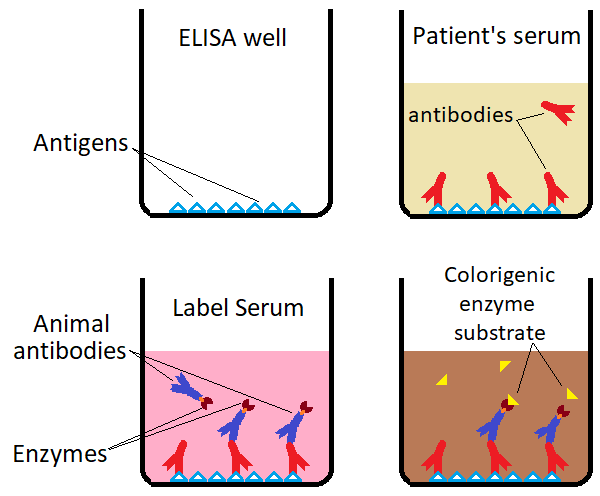
\includegraphics[width=7cm]{ELISA_well.png}
    \caption{Operational steps of a conventional enzyme-linked immunosorbent assay (ELISA). In the top left, the walls of the ELISA well are incubated with antigens. The top right shows the target antibodies in the patient's serum binding to the antigens in the well. The well is then washed to remove unbound antibodies. In the subsequent step, the label serum containing enzyme-linked secondary antibodies is added. The secondary antibodies bind to the primary antibodies and the well is washed again to remove unbound secondary antibodies. Finally, the reagent is added to elicit a color change upon catalysis with the enzyme.}
    \label{fig:ELISA_well}
\end{figure}

In order to be useful as a biosensor, a silicon photonic waveguide must first be functionalized by coating its surface with receptor biomolecules \cite{swg1}. As in ELISA, these receptors must bind, with a high degree of specificity, to the analyte. For instance, a biosensor might be based on an antibody-antigen pairs, in which antibodies will only attach to their corresponding antigens. When a sample containing the analyte is placed in contact with the waveguide, the analyte binds to the surface receptors, causing a change to the local index. The presence of analytes is then inferred by the corresponding change in output signal. Thus, the \textit{specificity} of photonic biosensors depends on the choice of surface receptors, while the device's \textit{sensitivity} depends on the geometric implementation of the photonic waveguides. We will focus on the latter, particularly on how SWG ORRs are able to achieve much higher sensitivities than other designs.

\vspace{-1em}
\section{III. Subwavelength grating waveguides}
\vspace{-1em}

While conventional strip waveguides consist of a high refractive index core, SWG waveguides consist of an alternating arrangement of high-refractive index and low-refractive index segments \cite{OGswg}. FIG. \ref{fig:SWGdiagram} illustrates an SWG waveguide formed by a periodic arrangement of high-refractive index Si embedded on low-refractive index SiO$_2$ substrate. The SWG is characterized by a height $H$, width $W$, grating period $\Lambda$, and duty cycle $DC= L_\text{Si}/\Lambda$, where $L_\text{Si}$ is the length of the high-refractive index material (silicon) measured in the direction of propagation. 

\begin{figure}[!ht]
    \centering
    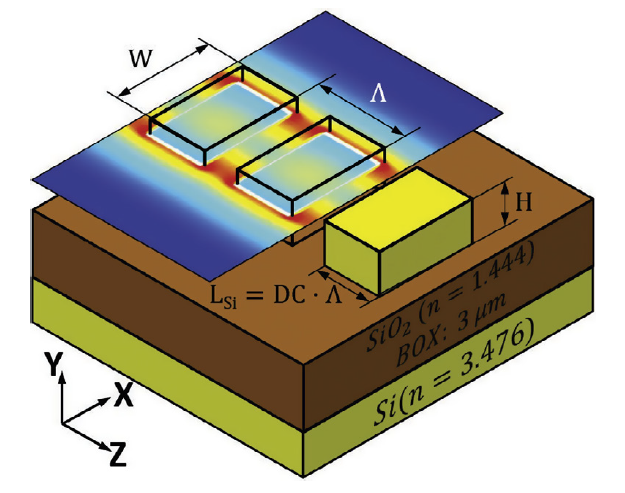
\includegraphics[width=6cm]{swgwaveguide2.png}
    \caption{From \cite{swg1}. Schematic of an SWG waveguide with constant pitch $\Lambda$ and duty cycle $DC = L_\text{Si}/\Lambda$. The electric field profile in the $xz$ plane is shown at $y = H/2$.}
    \label{fig:SWGdiagram}
\end{figure}

Electromagnetic fields in periodic grating waveguides excite Bloch-Floquet modes \cite{PhotonicCrystalsText}. These Bloch-Floquet modes are the natural modes of periodic media, and have mechanics that can be treated analogously to electron wavefunctions in a periodic crystal structure. In particular, the electric field of a Bloch-Floquet mode propagating through a uniform-period grating in the $\hat{z}$ direction can be described by $E(x,y,z+\Lambda) = E_B(x,y,z)e^{-\gamma_B\Lambda}$, where $E_B(x,y,z)$ is the Bloch mode field distribution within a single period $\Lambda$, and $\gamma_B$ is the associated complex propagation constant. In general, $\gamma_B = \alpha_B + jk_B$, and $k_B = (2\pi/\lambda)n_B$, where $\alpha_B$ is the attenuation constant, $k_B$ is the propagation constant, and $n_B$ is the effective index of the Bloch-Floquet mode \cite{HalirReview}. 


For a given grating pitch $\Lambda$, the behavior of a periodic waveguide depends strongly on the free-space wavelength $\lambda$. In particular, depending on $\overline{\lambda} = \lambda/\Lambda$ (i.e. the ratio of free-space wavelength to grating pitch), the waveguide can operate in one of three regimes: (i) diffraction, in which the waveguide segments scatter an incoming beam away from the waveguide; (ii) reflection, in which an input beam from a conventional strip waveguide is reflected back into the input and gradually attenuated in the periodic waveguide; (iii) subwavelength, in which diffraction and reflection effects are suppressed \cite{HalirReview}. 

 \begin{figure}[!h]
    \centering
    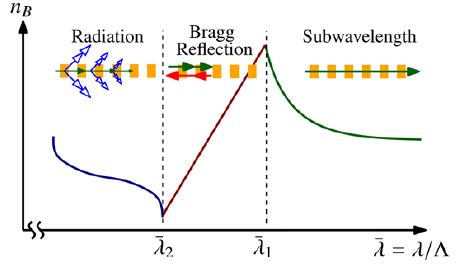
\includegraphics[width=7cm]{swgoperation.png}
    \caption{From \cite{HalirReview}. Bloch-Floquet mode effective index ($n_B$) as a function of the wavelength-to-pitch ratio $\overline{\lambda} = \lambda/\Lambda$.}
    \label{fig:SWGoperation}
\end{figure}

\pagebreak

\onecolumngrid

 \begin{figure}[!ht]
    \centering
    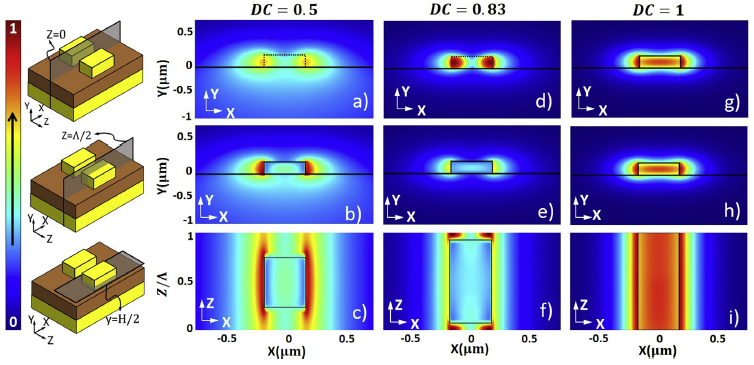
\includegraphics[width=15cm]{swgfield.png}
    \caption{From \cite{swg1}. Electric field distribution for various duty cycles with $W=350$ nm, $H=220$ nm, and $\Lambda = 250$ nm. The case of $DC=1$ corresponds to a conventional strip waveguide.}
    \label{fig:swgfield}
\end{figure}

\twocolumngrid

As shown in FIG. \ref{fig:SWGoperation}, light is radiated away from the waveguide for wavelengths comparable to the pitch of the grating (i.e. $\lambda/\Lambda <\overline{\lambda}_1$). Within the bandgap ($\overline{\lambda}_1<\overline{\lambda}<\overline{\lambda}_2$), the effective index follows the linear relation $n_B^{\text{Bragg}} \sim \frac{1}{2}\overline{\lambda}$. The subwavelength operating regime is reached when $n_B$ drops below the Bragg condition such that $n_B<n_B^{\text{Bragg}}$ \cite{HalirReview}. In this regime, diffraction and reflection effects are suppressed, and the SWG structure admits light as if it were a homogeneous waveguide. While conventional strip waveguides have strong optical confinement due high cladding-core index contrast, SWG waveguides have more field delocalization, with a greater proportion of the propagating signal residing outside of the core waveguide material. More precisely, the field profile reaches further into the waveguide's cladding region as shown in FIG. \ref{fig:swgfield}. For the application of biosensing, this translates to a higher modal field overlap with the analyte, resulting in increased sensitivity \cite{EvFieldBio}.

\section{IV. Optical Ring Resonators and sensor performance metrics}
\vspace{-1em}

An optical ring resonator (ORR) is said to be ``on resonance'' when the propagating wavelength fits an integer number of times inside the optical length of the ring cavity \cite{sipORRs}. In other words, 
\begin{equation}
    \lambda_\text{res} = \frac{2\pi r n_\text{eff}}{m}, \qquad m \in \mathbb{Z}^+,
    \label{eq:lamdares}
\end{equation}
where $r$ is the radius of the ring and $n_\text{eff}$ is the effective index of the guided mode. When an input waveguide is placed in close proximity to an ORR, the incoming signal will selectively couple from the waveguide to the resonator, depending on if the wavelength of the signal satisfies the resonance condition of the ORR.

Molecular binding, which occurs when analytes come into contact with an appropriately functionalized surface, causes a change in the local effective index, thus inducing a change in the ORR's resonant wavelength, as evident from equation \eqref{eq:lamdares}. By examining the shift in $\lambda_\text{res}$, we can determine the concentration of a given analyte in the sample. In order to do this, we must first define several metrics. The most important metrics for quantifying ORR sensor performance are as follows: (1) Sensitivity ($S$), (2) Resonator Quality Factor ($Q$), and (3) the Limit of Detection (LoD) \cite{sipresonators}. The remainder of this section is concerned with the description of each of these metrics.

\vspace{-1em}
\subsection{1. Sensitivity ($S$)}
\vspace{-1em}

We can quantitatively define sensitivity as having two components, $S= S_aS_w$. The first component, $S_a$ is attributed to the architecture of the sensing device, while the second component, $S_w$, is attributed to the waveguide mode sensitivity. For ring resonators, the architecture sensitivity is given by $S_a = \frac{\lambda_\text{res}}{n_g}$ \cite{swg1}, where $n_g$ is the group index, which can be obtained from the ring's free spectral range ($FSR$) by: $n_g = \frac{\lambda_\text{res}^2}{2\pi r \cdot FSR}$ \cite{swg3}.

The waveguide sensitivity parameter $S_w$ serves to map the process of molecular binding to variations in the effective index, $n_\text{eff}$. In particular we define:
\begin{equation}
    S_w = \frac{\partial n_\text{eff}}{\partial \Gamma},
    \label{eq:Sw}
\end{equation}
where $\partial \Gamma$ is the variation of a physical parameter of interest \cite{sipresonators}. Typically, $\Gamma$ either refers to the refractive index of the cladding, $n_c$, or the effective thickness of the adsorbed biomolecular layer, $t_\text{ad}$.

The case in which $\partial \Gamma = \partial n_c$ in equation \eqref{eq:Sw}, is referred to as the waveguide bulk sensitivity, $S_{w,b} = \frac{\partial n_\text{eff}}{\partial n_c}$. The total bulk sensitivity, being the change in resonant wavelength ($\Delta \lambda_\text{res}$) per unit change in refractive index of the cladding ($\Delta n_\text{clad}$), can then be expressed as follows \cite{swg3}:
\begin{equation}
    S_b = \frac{\Delta \lambda_\text{res}}{\Delta n_\text{clad}} = \frac{\lambda_\text{res}}{n_g}\left(\frac{\partial n_\text{eff}}{\partial n_\text{clad}}\right) \qquad \left[\frac{\text{nm}}{\text{RIU}}\right].
    \label{eq:Sbulk}
\end{equation}
Alternatively, the case in which $\partial \Gamma = \partial t_\text{ad}$ is referred to as the waveguide surface sensitivity,  $S_{w,s} = \frac{\partial n_\text{eff}}{\partial t_\text{ad}}$. The total surface sensitivity, being the change in the resonant wavelength ($\Delta \lambda_\text{res}$) per unit change in the effective thickness of the adsorbed biomolecular layer ($ \Delta t_\text{ad}$), can then be expressed as follows:
\begin{equation}
    S_s = \frac{\Delta \lambda_\text{res}}{\Delta t_\text{ad}} = \frac{\lambda_\text{res}}{n_g}\left(\frac{\partial n_\text{eff}}{\partial t_\text{ad}}\right) \qquad \left[\frac{\text{nm}}{\text{nm}}\right].
    \label{eq:Ssurf}
\end{equation}

While these electromagnetic definitions of sensitivity are useful to a photonic systems designer, they can also be made useful from a biochemical perspective \cite{swg1}. In particular, we can map the waveguide bulk sensitivity as $S_{w,b} \to \frac{\partial n_\text{eff}}{\partial c}$, where $\partial c$ is the variation in molar concentration with units of moles per liter $\left[M\right]$. This results in a total bulk sensitivity with units of $\left[\frac{\text{nm}}{M}\right]$, interpreted as the resonant wavelength shift per unit change in molarity. Similarly, we can map the waveguide surface sensitivity can as $S_{w,s} \to \frac{\partial n_\text{eff}}{\partial \rho_s}$, where $\partial \rho_s$ is the variation in mass surface density of the adsorbed layer with units of $\left[\frac{\text{pg}}{\text{mm}^2}\right]$. This results in a total surface sensitivity with units of $\left[\frac{\text{nm}}{\text{pg}/\text{mm}^2}\right]$, interpreted as the resonant wavelength shift per unit change in adsorbed layer mass surface density.

In practice, not all binding sites are uniformly occupied by a target molecule. Therefore, the effective thickness is modulated by the concentration of the our target molecule in the cladding. As a result, the notion of an ``effective'' thickness is defined as:
$t_\text{ad}$ = $L\frac{n_o}{n_e+n_o}$, where $n_o$ and $n_e$ are the number of occupied and empty binding sites, and $L$ is the length of the molecule measured perpendicularly from the binding site. This phenomenon is often difficult to simulate, and many authors (\cite{swg3, EvFieldBio,labelfree,sipresonators}, \textit{et. al.}) opt to use the bulk sensitivity.
\vspace{-1em}
\subsection{2. Resonator Quality Factor ($Q$)}
\vspace{-1em}
The resonator quality factor $Q$ is a measure of the sharpness of resonances in the optical transmission spectrum. In particular, $Q = \frac{\lambda_\text{res}}{\Delta \lambda_{3\text{dB}}}$, where $\Delta \lambda_{3\text{dB}}$ is the resonance 3 dB linewidth. The $Q$ factor is physically related to the optical confinement factor and the amount of energy lost per cycle. Since conventional strip waveguides have higher confinement factors and lower propagation losses compared with SWG waveguides, they are more efficient in terms of power. These effects translate to conventional strip ORRs having higher $Q$-factors, meaning that the light circulates longer and interacts with the analyte over a greater number of circulations. However, since most of the energy travels inside the waveguide structure due to the high optical confinement, conventional strip ORRs are less sensitive to a changes in cladding refractive index. Thus, although conventional ORRs tend to have higher $Q$-factors, they tend to have lower bulk and surface sensitivities. 

\vspace{-1em}
\subsection{3. Limit of Detection (LoD)}
\vspace{-1em}

The significance of the trade-off between sensitivity, $S$, and quality factor, $Q$, becomes apparent when considering the biosensor's limit of detection (LoD), which is the minimum amount of detectable variation in the physical parameter $\Gamma$ from equation \eqref{eq:Sw}. For a variation $\partial \Gamma$ that causes the minimum detectable resonance shift $\Delta \lambda_\text{min}$, the LoD is given by $\text{LoD} = \frac{\Delta \lambda_\text{min}}{S}$, where $S$ can refer to either bulk sensitivity $S_b$ or surface sensitivity $S_s$. When comparing the performance of different resonant sensors, a more useful metric is the intrinsic limit of detection (iLoD), which is defined by setting the system resolution to the resonance 3 dB linewidth $\Delta \lambda_\text{3dB}$. In other words, \begin{equation}
\text{iLoD} = \frac{\Delta\lambda_\text{3dB}}{S} = \frac{\lambda_\text{res}}{Q\cdot S} \qquad \left[\text{RIU}\right].
\label{eq:iLoD}
\end{equation}
Thus, the iLoD of equation \eqref{eq:iLoD} provides a means for quantitatively comparing the performance of strip ORRs and SWG ORRs, even while considering the trade-offs between sensitivity and $Q$-factor. 

\section{V. SWG Optical Ring Resonators} %SWGMR -> SWG ORR for consistency
\vspace{-1em}
The analytical approach for SWG ORRs is the effective refractive index method. As discussed in the section on SWG waveguides, there are 3 regimes of operation for periodic grating waveguides (radiation, reflection and subwavelength). For our purposes, we are interested in the subwavelength case. In this regime, waveguides behave as if they were a continuous waveguide with reduced refractive index ($n_\text{core-eq}$) \cite{swg3}. In particular, we have
\begin{equation}
    n_\text{core-eq} = n_\text{clad} + \eta \Delta n,
    \label{eq:n_eq}
\end{equation}
where $\eta$ is the duty cycle, and $\Delta n$ is the refractive index contrast:  $\Delta n = n_\text{core} - n_\text{clad}$. Using this method, we simplify the analysis of SWG ORRs, treating them as conventional continuous waveguides with reduced index. The reduced core-cladding index contrast results in one of the primary advantages: a greater proportion of the energy is carried outside of the core material. As a result, SWG ORRs have much greater sensitivities to changes in the cladding material. Although the reduced confinement is beneficial for biosensing sensitivity, it becomes problematic when considering bent waveguides, such as those that form ring resonators.

\pagebreak
% this needs to be at the top a page in the final version
\onecolumngrid

 \begin{figure}[!ht]
    \centering
    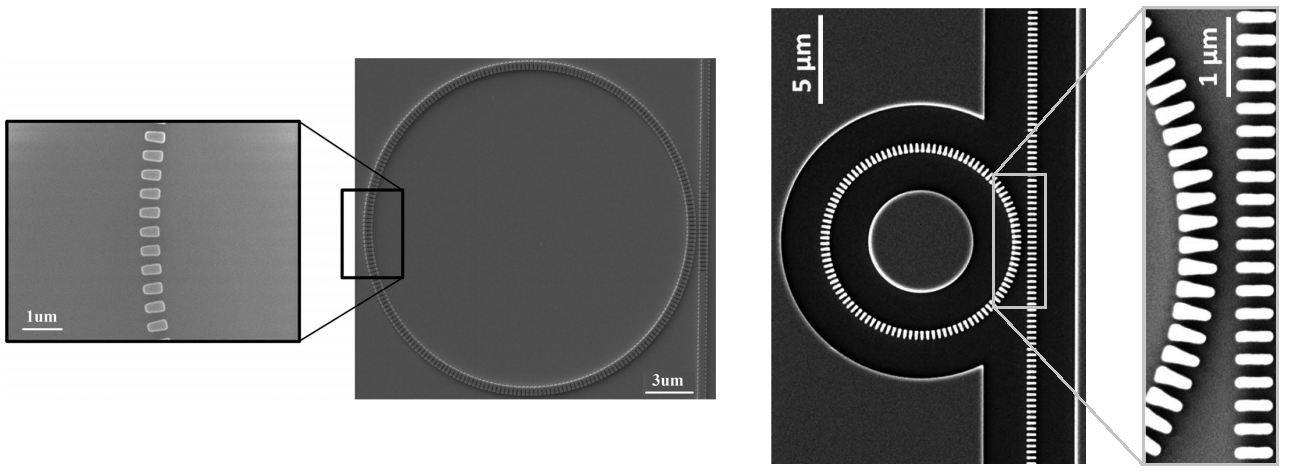
\includegraphics[width=15cm]{SWGSEM.png}
    \caption{\textbf{Left}: From \cite{swg3}. Scanning electron microscope image of one of the first SWG ring resonators used for biosensing. The structure was fabricated using electron beam lithography and is shown in air cladding. Segments have a grating period of 250 nm, duty cycle $\eta$ of 0.7,  an in-plane width of 500 nm, and an out-of-plane thickness of 220 nm.  \\ 
    \textbf{Right:} From  \cite{trapezoidal}. Scanning electron microscope image of a 5 $\mu$m radius T-SWG ORR. The structure was fabricated using electron beam lithography and is shown in air cladding. Segments have a length of 500 nm, long width of 210 nm, short width of 140 nm, and out-of-plane thickness of 250 nm.}
    \label{fig:swgSEM}
\end{figure}

\twocolumngrid

While all ORRs experience bend losses, losses with SWG ORRs is noticeably higher due to their lower optical confinement. This higher bend loss directly results in significantly lower $Q$-factors. One way to mitigate unacceptable bend loss is to tune the rectangular geometry of the segments in the ring structure. In particular, experimental results with trapezoidal silicon pillars (henceforth referred to as T-SWG ORR), have demonstrated the possibility to significantly reduce the bend loss by introducing an effective index asymmetry \cite{trapezoidal}. The side-by-side scanning electron microscope image in FIG.\ref{fig:swgSEM} illustrates the difference between rectangular pillar and trapezoidal pillar SWG ORRs. For ORRs of similar size, the T-SWG design maintains both high Q factor and high sensitivity when compared with rectangular segment SWG ORRs. As a result, T-SWG ORRs can be built using a smaller chip surface area as compared with rectangular SWG ORRs for similar $Q$, $S$, and iLoD requirements. 



%As we can see the trapezoidal pillars take advantage of the Snell's law to better guide the wave travelling through the ORR, bending it slightly with each segment it passes. In doing so, bend losses are minimized \cite{trapezoidal}.All this is made possible because of the decreased bending loss combined with the SWG design which allows the wave to travel in the cladding while remaining guided, making the modes more sensitive to changing refractive indices with bend losses much lower than those observed in rectangular SWG ORRs.






\section{VI. Practical Implementations}
\vspace{-1em}

%  In addition, we compare the performance of the T-SWG ORR design with that of the conventional rectangular (R-SWG) ORR design. In addition, to ensure the effectiveness of subwavelength grating micro-ring resonator (SWGMR) devices we must look at how the analytical results compare to the simulated system results, and more importantly how experimental results conducted in the real world measure up to the analytical and simulated approximations.

In this section, we compare various ORR designs. In particular, we discuss the experimental results of several ORR implementations. We pay particular attention to T-SWG ORRs, as these have shown exceptional promise due to their combination of high $Q$ factor and high sensitivity, leading to lower (better) iLoDs.

% I think we can only include the experimental results -- this would cut down on our word count and save time making the tables

%As we would expect simulations yielded nearly identical results as the analytical approaches. What may be surprising is the fact that experimental results of sensitivities fell short of the latter approaches as discussed in \cite{swg3}. The reasons for this are simply the imperfections that occur when manufacturing such small and delicate devices, and the uncertainties which accompany experiments. Nonetheless, the result for iLoD (our best metric for biosensor performance, as discussed in previous sections) was on the order of twice the theoretical value (exp: $5.5\cdot 10^{-4}$; th: $2.4\cdot 10^{-4}$)\cite{swg3}. Despite the disconnect between the experiments and theory we still have a good approximation of the iLoD from theoretical methods. A good rule of thumb would be to double the theoretical iLoD for results you would get in practice.

%This comes as no surprise since SWGs allow guided modes to travel in the cladding and thus interact more directly with the analyte.

When looking at the performance of ORR designs shown in TABLE \ref{tab1}, it becomes apparent that the interaction of SWG devices with the cladding material plays a significant role in improving results. SWG ORRs designed in \cite{swg3} show an almost 2-fold sensitivity increase when compared to the best TM mode strip ring resonators \cite{StripBiosensor}. In addition, SWG designs \cite{swg3, TSWGbio, MultiboxSensor} exhibit higher sensitivities than slot waveguides \cite{SlotBiosensor}.
\pagebreak
\begin{table}[!h]
\centering
\begin{tabular}{|c|c|c|c|c|}
\hline
\textbf{Sensor Type} & \textbf{$Q$-factor} & \textbf{$S_b \quad \left[\frac{\text{nm}}{\text{RIU}}\right] $} & \textbf{iLoD $\left[\text{RIU}\right]$} & \textbf{Ref.} \\ \hline
Strip ORR (TE) & 20000 & 70 & 0.00111 & \cite{TEsensor} \\ \hline
Strip ORR (TM) & 10778 & 228 & 0.00063 & \cite{StripBiosensor} \\ \hline
Slot ORR & 1800 & 298 & 0.00372 & \cite{SlotBiosensor} \\ \hline
Disk Resonator & 131000 & 21 & 0.00055 & \cite{DiskSensor} \\ \hline
Multibox SWG & 2500 & 580 & 0.00103 & \cite{MultiboxSensor} \\ \hline
SWG & 7000 & 405 & 0.00056 & \cite{swg3} \\ \hline
T-SWG & 9100 & 440.5 & 0.00039 & \cite{TSWGbio} \\ \hline
\end{tabular}
\caption{Tabulated experimental results from several ORR designs. The resonators have radii varying between $10$ and $30$ $\mu$m, with specific dimensions and design parameters available in the corresponding references.}
\label{tab1}
\end{table}

While SWG ORRs indeed have higher sensitivities, they are less competitive when considering the device's $Q$-factor. This is highlighted by the multibox SWG designed by \cite{MultiboxSensor}, in which the waveguide is composed of nanoscale segments in both the propagation and crosswise directions. While the multibox SWG design exhibits the highest sensitivity due to its low mode confinement, it also exhibits a very low $Q$-factor. The result is a higher (worse) iLoD than the SWG and T-SWG designs. In contrast, the disk resonator design \cite{DiskSensor}, in which the ORR consists of a high index disk, has a very high $Q$-factor due to the strong optical mode confinement. However, this strong confinement leads to a very low device sensitivity and an iLoD comparable to the SWG ORR design. 

When considering the design of future ORR biosensors, we see much promise in the geometrically tuned T-SWG ORR design. As shown in TABLE \ref{tab1}, the T-SWG exhibits a slightly higher sensitivity than the SWG ORR, while maintaining a higher $Q$-factor. When using the iLoD as the evaluation metric, we see that the T-SWG design outperforms all other designs. In particular, the T-SWG design \cite{TSWGbio} achieved an iLoD of $3.9\cdot 10^{-4}$ RIU, which outperforms the SWG ORR, TM strip ORR, disk resonator designs, whose iLoDs have values of $5.6 \cdot 10^{-4}$ RIU, $6.3\cdot 10^{-4}$ RIU, and $5.5 \cdot 10^{-4}$ RIU, respectively. To achieve ELISA-level sensitivity, photonic biosensors must achieve iLoDs lower than $10^{-6}$. Such iLoDs correspond to the detection of analytes in concentrations of a few ng/ml \cite{LoDPhotonicBiosensors}. The best performing photonic resonator design, the T-SWG ORR, exhibits an iLoD of $3.9 \cdot 10^{-4}$ RIU, leaving two orders of magnitude before becoming competitive with ELISA's limit of detection \cite{ELISAlimit}.

% took out the specifications on dimensions for word count

%Furthermore, when the radius is decreased to 5 $\mu$m the trapezoidal pillars lead to a more than 4-fold increase in $Q$. In the case where the ORRs were made specifically for biosensing purposes (i.e. the cladding material was water), we can compare the experimental performances of T-SWG and R-SWG ORRs. What we find is that the optimal performance is achieved at radii of 10 microns and 30 microns for T-SWG and R-SWG devices respectively. The duty cycles and feature sizes were also slightly different.. In the end the T-SWG outperformed the R-SWG device by achieving a quality factor of 9,100 over 7,000, despite the reduced radius of curvature. In addition, the sensitivity of the T-SWG was 440.5 nm/RIU, beating the R-SWG sensitivity of 405 nm/RIU. This is all taken into account and summarized by the intrinsic Limit of Detection (iLoD), in which the trapezoidal pillar device achieved $3.9\cdot 10^{-4}$ versus the rectangular pillar result of $5.6 \cdot 10^{-4}$. Therefore, the significance of T-SWG ORRs to biosensing applications cannot be overlooked, it produces greater experimental resolution even when confined to a smaller area than its R-SWG counterpart.

One important consideration for silicon photonic biosensors is the limitation imposed by the fabrication process. Current foundry processes available to silicon photonics have feature resolution limits of around 100-150 nm \cite{cmos}. This limitation is especially problematic for SWG designs, which often require minimum feature sizes in the range of 50-80 nm \cite{swg1}. While this resolution is achievable with electron beam lithography, the process is both lengthy and costly. Until a high resolution scalable foundry process becomes available to silicon photonics, SWG ORR biosensors face difficulty in overcoming solid core designs and becoming a frontline diagnostic device. 



\section{VII. Conclusion}
\vspace{-1em}
%As silicon photonicdevices are compatible with existing CMOS foundry processes, ORR biosensors are well-suited for the front-line of real-time medical diagnostics, such as early detection, drug testing, blood typing, and more. 

While there is still room for improvement, silicon photonics provides a platform for tremendously powerful fast, real-time, multiplexed interrogation comparable with current diagnostic methods. Although the limits of detection are not yet low enough to be competitive with the most sensitive conventional assay units, silicon photonic biosensors have considerable potential to displace the ELISA test. In the near future, we might expect to see photonic biosensors for applications which do not need very low limits of detection, such as blood typing and certain disease screening. 

In addition to requiring a full laboratory and trained technician to perform an ELISA test, the lengthy process of serial dilution makes the ELISA process both costly and lengthy. But perhaps the most important advantage of silicon photonics is the elimination of the need for costly label serums. When combined with on-chip light sources and photodetectors, label-free biosensing with silicon photonics has potential for scalable home diagnostics. One can imagine a future in which portable diagnostic devices based on photonic integrated circuits are commonplace for rapid on-site diagnosis. Despite the current limitations in fabrication and sensitivity, the future is bright for silicon photonic biosensing.

%The major advantage of this technology would come in photonic integration, when multiple assays can be multiplexed onto a single chip that would have the ability to detect multiple target molecule concentrations in parallel and return results in a few seconds; as opposed to conventional assays, such as ELISA, which require hours of work by a technician to determine a single concentration. 

%In addition, assays like ELISA require label serums to indicate the concentration or presence of a molecule, the need for this extra reagent could be eliminated by label-free biosensing, such as silicon photonics. The major drawbacks remain as: fabrication of application specific photonic integrated circuits, and the iLoD being much larger than that of ELISA. However, most tests do not require pg/mL levels of precision and ng/mL precision, as is achievable with T-SWG ORRs, would be sufficient.

%T, and at the forefront we expect to see T-SWG ORR biosensors greatly improving the speed of medical assays without greatly sacrificing precision.


% commented sections are more summary-like than conclusion-like. The conclusion should be more about future outlook of the technology, next steps in research, etc.

%In the early sections, we showed theoretical reasons why Sub-Wavelength Grating (SWG) ORRs have the advantage over conventional continuous waveguides in biosensing applications. Specifically, we showed how SWG ORRs guide light outside the core material, therefore making our waveguide much more sensitive to a change in the cladding's refractive index. We showed how the best way to classify biosensors is through the intrinsic Limit of Detection (iLoD), since it takes into account both the quality factor ($Q$) and the sensitivity ($S$) which are often inversely related, since they depend on optical confinement in opposite ways. 

%In the analysis, we found that our predictions were correct with regard to the increased sensitivities of SWG ORRs versus the continuous ORRs, however with a sacrifice in the quality factor. Overall, the best results came out of the trapezoidal pillar (T) variation of SWG ORR devices in which the geometry allowed for higher Q-factors by minimizing bending loss without any considerable loss in sensitivity since the wave still travels through the cladding material. This translated to T-SWG ORRs having the smallest iLoD of any waveguide biosensor we found, specifically $3.9*10^\text{-4}$ RIU. Because of imperfections in the fabrication process we are still removed from the theoretical minimum iLoD of $2.4*10^\text{-4}$ RIU, which would be sufficient to replace ELISA (the predominant labelled biosensor) in terms of precision. 




\bibliographystyle{IEEEtran}
\bibliography{mybib}

\section{Statements of Contribution}
\noindent D.H. wrote sections III, IV, and V.

\noindent S.L. wrote sections IV, V, and VI.

\noindent Y.L wrote section I, II, and III.

\noindent All authors reviewed the document and contributed equally to the final version.
\vspace{-1em}


\end{document}
